\documentclass[a4paper,12pt,oneside,openright]{article}
\usepackage[pdftex] {graphicx}
\usepackage[utf8]{inputenc}
\usepackage{listings}
\usepackage{graphicx}
\usepackage{chapterbib}

\usepackage{algorithm}
\usepackage{algorithmic}

\addtolength{\hoffset}{-1cm}
\addtolength{\textwidth}{2.5cm}

\lstdefinelanguage{J}[]{C}
{morekeywords={},
sensitive=false}
\lstset{language=J}
% shadowbox come frame
% rulesepcolor=\color{Gray}
\lstset{frame=trBL}
\lstset{frameround=fttt}
\lstset{tabsize=3, breaklines, commentstyle=\texttt}
\lstset{showstringspaces=false}
\lstset{basicstyle=\small}
\lstset{emph={},emphstyle=\textit}

\title{Performance evaluation of parallel sorting algorithms on large data sets}
\author{Nicola Desogus, Paolo Giangrandi, Fabio Luporini}

\begin{document}
\maketitle
\tableofcontents
\pagebreak

\section{Introduction}
This project has the aim of studying the well known problem of sorting \textit{atomic} items (i.e. they occupy O(1) space) within the context of parallel computing. All the standard sequential sorting algorithms can be re-designed to exploit parallel machines; as a matter of fact, literature is not poor of this kind of works. There are some sequential algorithms (such as mergesort or quicksort) that can be easily adapted to the new parallel context; nevertheless, other ones needs a trickier re-engineering. On the other hand, algorithms that performs very well on sequential machines could not be so good in their new parallel version. Thus, the first objective of this project is to sperimentally compare the performance of the most known parallel sorting algorithms. 

In this scenario things get even more complicated from the fact that we have to manage very large data sets, i.e. our parallel algorithms sort terabytes of data. This means that some of the theoretical results achieved in the field of \textit{external memory sorting} will have to be compared with the ones that we will sperimentally obtain. Further, in order to keep implementation complexity limitated, we decide to not extends our algorithms for exploiting the presence of multi-disks eventually provided by the parallel architecture. 

In this complicated context the role of the test environment becomes crucial. Obvioulsy, we can not say neither that our algorithms will scale the same way on every possible parallel machine nor that results are meaningful only for a specifc machine. Hence, analyzing the results, we will have to consider even some fundamental architectural aspects. At a first glance, we have to take care of at least two macroscopic aspects: first, the possibility that the parallel machine is a hierarchycal systems (e.g. a cluster of shared memory nodes); second, the interconnection network of the nodes. In case of a hierarchycal system, if we will be able to find a way for exploiting the presence of shared memory, then we might achieve a very significative gain in terms of performance. Hence, depending both on the way we will exploit shared memory and the properties of the interconnection structure (bandwith, latency), we might get performance results more or less close to the ones we expected.

We will address all this issues both from a theoretical point of view and by implementing a structured framework. This document is organized as follows: first, we briefly explain which algorithms will be parallelized; second, we describe all the characteristcs of our framework; then, after having described the test environment, we will detail the implementation of our algorithms and, for each of them, we will analyze their performance. Finally, we will compare all the achieved results.

\section{Objectives, assumptions and algorithms}
\label{assumptions}
In the first part of our work we put a lot of efforts in deeply understanding the state of the art of parallel sorting algorithms. The first thing we noticed is the lack of an unified theory that asserts whether an algorithm is better than another; this is an obvious consequence of the absence of realistic cost models for parallel algorithms and architectures (e.g. both $PRAM$ and the more refined $LogP$ are too superficials to be considered significant. Second thing, the literature is rich of parallel algorithms conceived and engineered for \textit{specific machines}, so to be able to exploit peculiar features of the machine itself, e.g. the structure of the interconnection network. Just as examples we can cite~\cite{CSPA, CSPA2}, but with some googling we can really find a lot of papers or report on these themes. This approach is not obviously good because of at least two facts: the high designing complexity and the non-portability. Hence, in our project, even if the practical performance analysis will be done on a specific architecture, the parallel algorithms will \textit{not} be designed for that specific machine. In some sense, our approach is more close to~\cite{NPSA}.

We list the sorting algorithms that we are going to parallelize, all of them based on the Divide$\&$Conquer paradigm. Notice that, in general, the parallelization consist of ''exporting'' either the divide or the conquer phase to the ''process level''. Just as an example, in parallel Mergesort the distribution phase will be made between the processes of the parallel algorithm. 
\begin{enumerate}
\item Mergesort
\item K-Way Mergesort
\item Load-Balance Mergesort (and some variants) 
\item Quicksort
\item Bitonicsort
\item Bucketsort
\item Samplesort
\end{enumerate}
Examples of parallelization of $some$ of these algorithms can be find in literature. For instance, it is easy to find parallel versions of Mergesort, Quicksort, Samplesort, Bitonicsort. On the other hand, we notice the lack (or at least the poor availability) of informations regarding K-Way Mergesort and Load-Balance Mergesort. In any case, as we will better explain later, we re-implemented all the algorithms. Indeed, all the MPI implementations we found were really poor in terms of quality of code and do not take into account the possibility of having to sort large data sets, a problem which requires a specific analysis. Once implemented, we will compare the performance of these algorithms in terms of their efficiency, scalability and completion time, by playing on some degrees of freedom like the parallelism degree and the size of the data sets.  
 
In this section we will summarize the assumptions for this project, emerged during the several meetings.
\begin{itemize}
	\item{The work we need to do is to compare parallel sorting algorithms and to study how they behave. We early understood that to achieve such goal we were forced to collaborate in some way. We had to define a common framework in order to have comparable results. If any of us computed times in different ways, these wouldn't have been comparable. If any of us used a different strategy to sort data sequentially, or different optimization to sort data in principal memory or in disk, results would have been worthless, since the comparison would have mixed the performance of a parallel sorting algorithm with the performance of something else that regards sequential computation. This, besides, allowed us to do a better work, having a well structured framework which can be extended to many other algorithms with little work.}
	\item{We are not interested to study how sequential algorithms behave. We care only about the parallel part of our algorithms. The sequential part is always implemented using the \textit{qsort} POSIX standard function, and it does not matter if it works on primary memory only, rather than on secondary one. Sequential and parallel sorting are completely disjoint operations, which can be studied separately.}
	\item{Some algorithms natively begin, or end, with data centralized in a single process, while others begin or end with data distributed among all processes. For example mergesort begins with data distributed: any process sorts its piece fo data, and send it to another node that takes care of merging it, in order to end with data centralized on a single process. Quicksort, at the opposite, start with centralized data; the first process splits data and sends it to the other, in order to end up with distributed sorted data. For this reason and to mantain some homogenity among the algorithms we chose to always begin and end with centralized data. The algorithms that begin or end with distributed data will take care of scattering or gathering data, studying these extra (ie: unneeded by the algorithm, but needed by our common algorithm-testbed) operations separately from the rest of the computation.}
	\item{Since our platform is a clusted made of multicore nodes, we know that communication patterns between our several processes may weight a lot on the final performances. We will be looking for heuristical approaches to map processes in order to study what scenario will result in best performances due to communications between cores on different nodes, or on different parts of the single node.}
\end{itemize}


\section{Assumptions [draft]}
In this section we will summarize the assumptions for this project, emerged during the several meetings.
\begin{itemize}
	\item{The work we need to do is to compare parallel sorting algorithms and to study how they behave. We early understood that to achieve such goal we were forced to collaborate in some way. We had to define a common framework in order to have comparable results. If any of us computed times in different ways, these wouldn't have been comparable. If any of us used a different strategy to sort data sequentially, or different optimization to sort data in principal memory or in disk, results would have been worthless, since the comparison would have mixed the performance of a parallel sorting algorithm with the performance of something else that regards sequential computation. This, besides, allowed us to do a better work, having a well structured framework which can be extended to many other algorithms with little work.}
	\item{We are not interested to study how sequential algorithms behave. We care only about the parallel part of our algorithms. The sequential part is always implemented using the \textit{qsort} POSIX standard function, and it does not matter if it works on primary memory only, rather than on secondary one. Sequential and parallel sorting are completely disjoint operations, which can be studied separately.}
	\item{Some algorithms natively begin, or end, with data centralized in a single process, while others begin or end with data distributed among all processes. For example mergesort begins with data distributed: any process sorts its piece fo data, and send it to another node that takes care of merging it, in order to end with data centralized on a single process. Quicksort, at the opposite, start with centralized data; the first process splits data and sends it to the other, in order to end up with distributed sorted data. For this reason and to mantain some homogenity among the algorithms we chose to always begin and end with centralized data. The algorithms that begin or end with distributed data will take care of scattering or gathering data, studying these extra (ie: unneeded by the algorithm, but needed by our common algorithm-testbed) operations separately from the rest of the computation.}
	\item{Since our platform is a clusted made of multicore nodes, we know that communication patterns between our several processes may weight a lot on the final performances. We will be looking for heuristical approaches to map processes in order to study what scenario will result in best performances due to communications between cores on different nodes, or on different parts of the single node.}
\end{itemize}


\section{Structuring the framework}
\subsection{Design choices}
\subsection{Data generation}
\subsection{Performance evaluation}
\subsection{API}

\section{Test environment}
\subsection{MPI cost model}

\pagebreak

\section{Description and performance evaluation of the algorithms}
\subsection*{Terminology}
We briefly describe the terminology that we are going to use in this chapter. Our parallel algorithms have been implemented on top of MPI, thus they are composed by a set of $N$ processes, each of them having its unique identifier. According to the MPI terminology, we refer to a specific process by calling it $rank$ $x$, where $x \in N$ represents its identifier. The input sequence $S$ that has to be ordered is of size $n$. 

In order to define the \textit{efficiency} $\varphi$ of an algorithm, we have to introduce some parameters:
\begin{itemize}
\item $P$, the number of real processors of our machine; 
\item $m$, the number of steps of the algorithm;
\item $T_i$, the duration of step $i$ (in seconds);
\item $X_i$, a random variable which counts the number of real processors that contribute to the calculation during the step $i$.
\end{itemize}
Therefore, we can define the efficiency as:
\begin{center}
$\varphi = \frac{\sum_{i=0}^m \frac{E[X_i]}{P}}{m} = \frac{\sum_{i=0}^m E[X_i]}{P \times m} $
\end{center}
The efficiency is a formal tool to establish how much an algorithm exploits the parallelism degree of a machine. $\varphi \rightarrow 1$ means that the algorithm, in each step, tends to use all the available processor of the machine. Obviously, $\varphi \rightarrow 1$ does not means that the algorithm is ''good''; indeed, for such claim, the value of both $m$ and $T_i$ must be considered. For instance, we might have $\varphi \rightarrow 1$ and $T_i \rightarrow\infty$, meaning that each step requires a lot of time; or even worse, $m \rightarrow\infty$, meaning that the algorithm requires a lot of steps in which almost all the processors are involved.

As we said, a parallel sorting algorithm is composed of some steps of computation. During each step, a process can do basically three things, obviouslly not mutual exclusive each other:
\begin{itemize}
\item it can send data to other processes (the process is a \textit{sender} of that step)
\item it can receive data from other processes (the process is a \textit{receiver} of that step)
\item it can perform computation.
\end{itemize}

\subsection{Mergesort}
Mergesort is a well-known sorting algorithm based on the Divide$\&$Conquer paradigm. Thinking to a parallel version of Mergesort is therefore quite natural. First of all, $S$ is scattered among the $N$ processes. Each process locally sorts its own portion of $\frac{n}{N}$ elements, using a standard sequential sorting algorithm, like \textit{qsort}. At this point, a sequence of $\lceil \log_{2}{N} \rceil$ steps starts; in everyone of them, a \textit{distribution} phase precedes a \textit{merging} phase. The distribution phase is performed \textit{between different processes}: for instance, $rank$ $1$ sends its data to $rank$ $0$, while $rank$ $3$ to $rank$ $2$ and so on. On the other hand, the merging phase is done locally by all the processes that received a portion of datas. Figure~\ref{merge-dist} clarifies these concepts. Further, we observe that as its sequential counterpart, our version of mergesort needs an auxiliary array of size $n$. 
\begin{algorithmic}[1]  
	\medskip
	\STATE $Scatter( S, S\_local )$
	\STATE $qsort( S\_local )$
	\REPEAT 
		\STATE $distribution( S\_local )$
		\STATE $fusion ( S\_local )$
	\UNTIL $i < \log_{2}{N}$
	\medskip
\label{alg1}
\end{algorithmic}
Notice that steps $\lbrace 1, 2 \rbrace$ will be tipically perfermed by all our algorithms, not just by Mergesort. We conclude this overview by emphasizing that the \textit{distribution} of datas in each step can be handled in many different ways; that is, there are many possibile communication patterns between processes, that may lead to different performance behaviour (for instance, because of the change of the load on the interconnection structure) . We will address this important topic in a following section.

\begin{figure}[h]
        \centerline{
               \mbox{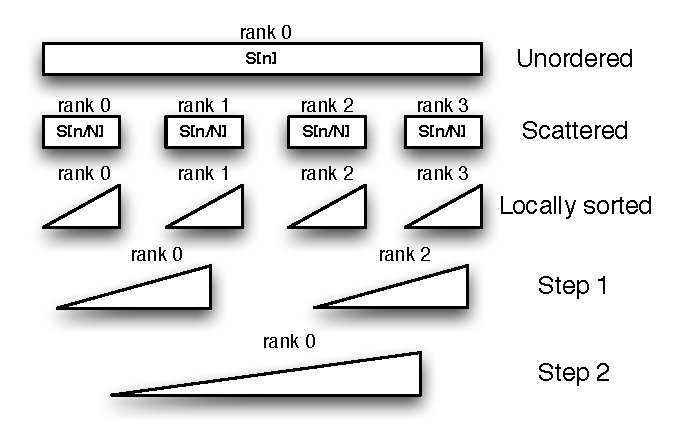
\includegraphics[scale=0.70]{mergesort-pict1}}
        }
        \caption{Parallel mergesort for $N = 4$.}
        \label{merge-dist}
\end{figure}

\subsubsection*{Parallel version}
\subsubsection*{Mapping virtual processors onto different cores} 
\subsubsection*{Performance Analisys} 
\subsubsection*{Efficiency} 
\subsubsection*{statistical analysys}

%\subsubsection{Parallel version}
%Descrizione della parallelizzazione dell'algoritmo; possibile uso di pseudocodice. Per lo pseudocodice ho definito in Relazione.tex un template da poter utilizzare. Ad esempio, se voglio includere lo pseudocodice del mergesore, basta scrivere: $lstinputlisting{mergesort.code}$. Per convenzione i file con lo pseudocodice scriviamoli con estensione .code.
%\subsubsection{Mapping virtual processors onto different cores} 
%only if they are considered in the specific version
%\subsubsection{Performance Analisys} 
%Qua discutiamo di completion time e quindi scalability ecc. Magari facciamo un confronto con quelle che devono essere le prestazioni ideali.
%\subsubsection{Efficiency} 
%Magari il nome di questa sezione va ''raffinato''..cmq, qua discutiamo di quello che diceva il coppola, cioè ad ogni step dell'ordinamento quanto riusciamo a sfruttare l'architettura parallela. Magari c soffermiamo su quanto la presenza del multicore sia effettivamente sfruttata e quanto. 
%\subsubsection{statistical analysys}
%to be discussed in case variance is high...questo magari possiamo scriverlo DOPO aver fatto i test.

\subsubsection{K-Way Mergesort}
\label{kmerge}
The idea of sequential K-Way Mergesort is to enhance the merging phase by enlarging to $K$ the number of runs that are fused at a time. This approach, designed in the context of external-memory model, aims at reducing the I/O-complexity of Mergesort by improving the memory space utilization~\cite{FERR}. 

We reuse this idea, but with different purposes, to get another parallel version of Mergesort: now, the objective is not to lower the I/O-complexity, but rather to improve the \textit{efficiency}, that is both to diminish the number of steps of the algorithm and to increase the number or computing processor at each step. An initialization phase takes place as in Mergesort: $S$ is scattered among the processes and it is locally sorted. With respect to Mergesort, the distribution phase needs to be modified. While in Mergesort, in each step, there were exactly many senders as many receivers ($\frac{\sharp senders}{\sharp receivers} = 1$), in K-Way Mergesort the number of senders is higher ( $\frac{\sharp senders}{\sharp receivers} = K - 1$, see figure~\ref{k-merge-dist}). In other words, in a specific step, a process may receive data from $K-1$ processes. This approach allows us to reduce $m$ with respect to Mergesort. The merging phase is performed locally by the processes that have received $K-1$ blocks of data during the step. From sequential K-Way Mergesort we know that the best way to implement the fusion of more than two runs is to use a Heap data structure~\cite{FERR}; since in our parallel context the merging phase is not modified, we re-adopt the same approach.

We notice that in K-Way Mergesort the average value of $T_i$ may be different from the one we obtained for Mergesort. This is may due both to a longer merging phase and to the potential conflicts that may arise on the interconnection structure when $K-1$ processes try to send data to the same specific process.

\begin{figure}[h]
        \centerline{
               \mbox{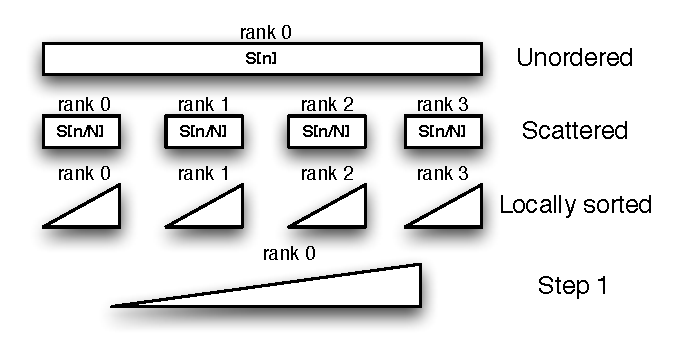
\includegraphics[scale=0.70]{kmerge-pict1}}
        }
        \caption{Parallel mergesort for $N = 4$, $K = 4$.}
        \label{k-merge-dist}
\end{figure}

\subsubsection*{Mapping virtual processors onto different cores} 

\subsubsection{Load-Balanced Merge Sort}
When we refer to load balancing, we ideally want all the processes to be operating continuously in the overall computation, which would lead to the minimum execution time. Achieving this goal by spreading the work evenly across processes is called load balancing.

The main limit of the classic approach in parallelizing merge sort is due to the number of idle processes that keeps growing during the merging phase. The active processes are halved at each step. Therefore, the maximum achievable efficiency is severely limited. The aim of the \textit{Load-Balanced Merge Sort} we implemented is to force each process to participate in the entire merging phase in order to obtain higher parallelism and increase efficiency.

To define the range of numbers on which a process will operate during the merge, a preprocessing phase is required. A regular sampling scheme is exploited to picks out $n-1$ numbers, $s_1$, $s_2$, \dots, $s_{n-1}$, from the input sequence $S$ as \textit{splitters}. At the end of the overall computation, the partition of process $i$ will contain elements $e$ for which $s_{i-1} \leq e < s_i$.

At this point, a loop of $\log (n)$ steps starts. At each step $i$, groups of processors of size $2^i$ (where $0 \leq i \leq \log(n)$) are defined. Each group is assigned a partner group and all processes of a group will exchange data only with processes of the paired one. The \textit{Send-and-Receive} MPI routine is exploited to decrease communication latency (ideally, only a $T_{setup}$ is paid) and avoid deadlocks. A different partner process from which to start exchanging data is defined for each process inside a group. At step $i$, a subset of $2^{i+1}-1$ splitters are used to identify which elements must be sent to the paired-group processes. Once a process has exchanged data with the partner group, a merge operation on the received data and the local data is performed.

A final gather operation is required to retrieve the whole sorted sequence at the root process.

\subsection{Load-Balanced Multi-Way Merge Sort}
Basically, the weak point of the previous algorithm is given by some redundancy in moving data among processes. In fact, during the merging phase some processes will receive data that doesn't belong to their assigned range, resulting in a waste of time both in communication and computation. By avoiding this redundancy we achieved increase in performance. An extended preprocessing phase is required to determine exactly which elements of the local data fall in what interval according to the $n-1$ splitters. Communications follow the same pattern as in \textit{Load-Balanced Merge Sort}, but a process will receive only numbers that lies within its range. At the end of the loop, only one \textit{n-way merge} is performed on the whole received data and the remaining local data.



\subsubsection*{Parallel version}
\subsubsection*{Efficiency} 
\subsubsection*{Statistical Analysys}

\subsection{Quicksort}
Quicksort, like Mergesort, is a very popular sorting algorithm, the most widely used on sequential architectures. The algorithm has been implemented in a clean way, separating three logical phases:
\begin{itemize}
	\item{\textit{scattering} phase: processes that have some data partition it (according to a randomly-chosen pivot), and send it to waiting processes.}
	\item{sequential sorting phase: any process sorts its own partition with a sequential partition.}
	\item{\textit{gathering} phase: processes send sorted data back, to rebuild the whole sorted array.}
\end{itemize}
We will not spend any time talking about the sequential sorting phase, since it is in common with all the other algorithms.
The \textit{scattering} and the \textit{gathering} phases, instead, are a bit tricky; they are not the simple, \textit{primitive} scatter and gather offered by MPI, since they need to do some more computation: our custom scattering phase needs to choose a pivot, partition the array according to the pivot, and send a whole partition away, while the gather knows exactly where to place the data it is receiving, since such data is one of the partitions, which has been sorted.
We chose to implement our scattering phase as a binary three: rank 0 will partition its data and send the second partition to a second process, and this will go on recursively until all of our processes get their data. The idea of implementing a linear scattering has been discarded because it would not have allowed a parallelization of the partitioning, which is the most expensive operation of the scattering phase.
The gathering phase has instead been implemented in a linear way: each process sends its sorted data to rank 0 which will read the data directly in the final array, without needing a further merging operation.

\subsubsection*{Parallel version}
\subsubsection*{Mapping virtual processors onto different cores}  
\subsubsection*{Efficiency} 
\subsubsection*{statistical analysys}


\subsection{Bitonic Sort}
\textit{Bitonic sort} is based on repeatedly merging two bitonic sequences to form a larger bitonic sequence. A bitonic sequence is a sequence of $M$ values, $a_0, a_1, a_2, \dots, a_{M-2}, a_{M-1}$, that can be divided into two subsequences, one monotonically increasing and the other monotonically decreasing
\[
a_0 < a_1 < a_2 < \dots < a_i > a_{i+1} > \dots > a_{M-2} > a_{M-1}
\]
where $0 \leq i < M$.
A sequence is also considered bitonic if the preceding can be achieved by shifting the values cyclically.

On a bitonic sequence can be applied the operation called \textit{bitonic split} which halves the sequence in two bitonic sequences such that all the elements of one sequence are smaller than all the elements of the other sequence. Thus, given a bitonic sequence we can recursively obtain shorter bitonic sequences using bitonic splits, until we obtain sequences of size one, at which point the input sequence is sorted. The bitonic split is just a \textit{compare-and-exchange} operation on the $a_i$ and $a_{i+M/2}$ values (where $0 \le i < M$).

To sort an unordered sequence, the first step is to convert the $M$ numbers into a bitonic sequence with $\frac{M}{2}$ numbers in ascending order and $\frac{M}{2}$ numbers in descending order. This is done recursively by a compare-and-exchange operation on pairs of adjacent sequences (initially formed by only one element) obtaining bitonic sequences of larger and larger lengths. In the final step, a single bitonic sequence is sorted into a single increasing sequence.

This algorithm can be parallelized using $n$ processors as follows:
\begin{enumerate}
	\item the input sequence $S$ is scattered among processes;
	\item each process $A$ sorts locally its own partition of $\frac{M}{n}$ elements of the input sequence;
	\item at this point a loop of $\log(n)$ steps starts; at the $i$-th step:
		\begin{itemize}
			\item process $A$ communicates with the process $B$ whose rank differs from $A$'s rank only at the $j$-th bit;
			\item $A$ sends its own partition to $B$ and viceversa;			
			\item both processes perform a \textit{compare-and-exchange} operation on the received partition and the local one to produce two sequences of $\frac{M}{n}$ elements in which all the elements of one sequence are smaller than all the elements of the other sequence;			
		\end{itemize}
	\item the sorted sequence is gathered to the root process.
\end{enumerate}
Two auxiliary arrays (one to receive data and one to temporary hold the merging result) of size $\frac{M}{n}$ will be necessary.


%The pseudocode of the algorithm follows:
%\lstinputlisting{bitonicsort.code}



%\newtheorem{prop}{Propiet\'a}
%
%\begin{prop}
%asd
%\end{prop}
%
%
%
%\begin{description}
%	\item Esiste un indice $i$ (dove $0 \leq i \leq n-1$ ) tale che
%\end{description}

\subsubsection*{Parallel version}
\subsubsection*{Efficiency} 
\subsubsection*{Statistical Analysys}
\subsection{Bucket Sort}
\textit{Bucket sort} is not based upon compare and exchange, but is naturally a partitioning method. The idea behind bucket sort is that if we know the range of our elements to be sorted, say $0$ to $a-1$, we can divide this interval into $n$ equal regions, $0$ to $\frac{a}{n}-1$, $\frac{a}{n}$ to $2\frac{a}{n}-1$, \dots , and one bucket is assigned to hold values that fall within each region. The numbers are simply placed into the appropriate buckets and each bucket is sorted using the best sequential algorithm. However, bucket sort only works well if the original numbers are uniformly distributed across the known interval. 

To identify the region in which a number lies is sufficient to divide the number by $\frac{a}{n}$ and use the result as index of the proper bucket. Thus, placing all numbers into the buckets will require $M$ steps. If the numbers are uniformly distributed, there should be $\frac{M}{n}$ numbers in each bucket. The lower bound on any compare and exchange sorting algorithm on $k$ numbers is about $k \log k$ comparisons. Therefore, in the best case, to sort $\frac{M}{n}$ numbers of one bucket will require $\frac{M}{n} \log \frac{M}{n}$ steps. Let us assume that the concatenation of the sorted buckets takes no additional steps. Thus, the sequential time complexity of bucket sort becomes
\[
O( n \log \frac{M}{n} )
\]

Parallelizing bucket sort is straightforward. We will have $n$ processes, and as many buckets. Each process separates the numbers in its region into $n$ ``small'' buckets. These small buckets are then sent to the corresponding process (bucket $i$ process $i$) with an ``all to all'' communication. Thus, the algorithm follows these phases:
\begin{enumerate}	
	\item the input sequence $S$ is scattered among processes;
	\item each process separates the numbers in its partition into $n$ ``small'' buckets;
	\item each process sends the numbers in the ``small'' bucket $i$ to the process with rank $i$ (where $0 \leq i < n$);
	\item each process sorts locally its own bucket;
	\item the sorted sequence is gathered to the root process.
\end{enumerate}

 
\subsubsection*{Parallel version}
\subsubsection*{Performance Analisys} 
\subsubsection*{Efficiency} 
\subsubsection*{Statistical Analysys}
\subsubsection{Sample Sort}
The main problem in bucket sort is that the range of numbers for each bucket is fixed a priori. Thus, if numbers are not equally distributed, more numbers will fall into some buckets than others.
The goal of \textit{sample sort} is to determine the ranges so that each bucket will have approximately the same number of elements. To achieve this it uses a sampling scheme which picks out $n-1$ numbers, $s_1$, $s_2$, \dots, $s_{n-1}$, from the input sequence $S$ of $M$ elements as \textit{splitters}, that define the range of numbers for each of the $n$ buckets. Bucket $i$ gets the elements $e$ for which $s_{i-1} \leq e < s_i$. The selection of these splitters is a crucial issue. These can be found by the following method:
\begin{enumerate}	
	\item the input sequence $S$ is divided into $n$ partition each of $\frac{M}{n}$ elements;
	\item each partition is sorted and a sample of $n-1$ evenly spaced numbers is chosen from each of them;
	\item the obtained $n \cdot (n-1)$ samples are then sorted, and again $n-1$ equally spaced numbers are selected as global splitters;
\end{enumerate}
After the range of each bucket is set by the splitters, the algorithm continues in the same fashion as bucket sort, with the only difference in placing the numbers in small buckets, operation that now requires for each element a binary search on the array of splitters.

The parallel version of the algorithm works as follows:
\begin{enumerate}	
	\item the input sequence $S$ is scattered among processes;
	\item each process sorts its partition and selects a sample of $n-1$ evenly spaced numbers;
	\item the obtained $n \cdot (n-1)$ samples are gathered to the root process and then sorted;
	\item the root process selects $n-1$ equally spaced numbers as global splitters and broadcast them;
	\item each process separates the numbers in its partition into $n$ ``small'' buckets by performing a binary search on the array of splitters;
	\item each process sends the numbers in the ``small'' bucket $i$ to the process with rank $i$ (where $0 \leq i < n$);
	\item each process sorts locally its own bucket;
	\item the sorted sequence is gathered to the root process.
\end{enumerate}

 

\subsubsection*{Parallel version}
\subsubsection*{Efficiency} 
\subsubsection*{Statistical analysis}


\section{Comparing the algorithms: analysis of the results}

\section{Conclusions and future works}


                                                                    

%\lstinputlisting{mapreduce_types.code}

%\begin{figure}
%        \centerline{
%               \mbox{\includegraphics[scale=0.88]{CompletionTime_64}}
%        }
%        \caption{The completion time for the benchmark using a matrix of 64MB.}
%        \label{CompletionTime64}
%\end{figure}


\pagebreak

\begin{thebibliography}{13}
\bibitem{FERR}{Paolo Ferragina. \textit{The magic of Algorithms!.} Lectures notes in Algorithm Engineering, 2010}
\bibitem{CPSA}{Nancy M. Amato	 and Ravishankar Iyer and Sharad Sundaresan and Yan Wu.\textit{A Comparison of Parallel Sorting Algorithms on Different Architectures.} Technical Report 98-029, Department of Computer Science, Texas A$\&$M University, January 1996. }
\bibitem{CSPA2}{Marc Moreno Maza . \textit{CS855: Parallel Sorting Algorithms.} Technical Report, Department of Computer Science, The University of Western Ontario, February 2008.}
\bibitem{NPSA}{David R. Cheng and Alan Edelman and John R. Gilbert and Viral Shah. \textit{A Novel Parallel Sorting Algorithm for Contemporary Architectures.} In ALENEX06, May 2007.}
\end{thebibliography}
\end{document}
